\documentclass{article}
\usepackage[final]{pdfpages} %For using cover page pdf in the latex file
\usepackage[utf8]{inputenc}
\usepackage{geometry}
\usepackage{amsmath}
\usepackage{amsthm}
\usepackage{amsfonts}
\usepackage{amssymb}
\usepackage{graphicx}
\usepackage{tocloft}

%\usepackage{perpage} %the perpage package
%\MakePerPage{footnote} %the perpage package command

% For adding TOC in pdf bookmarks
\usepackage{hyperref}
\hypersetup{pdftex,colorlinks=true,allcolors=black}
\usepackage{hypcap}
%
\usepackage{float}
\usepackage{xepersian}
\usepackage{bidi}


\settextfont{Yas}
\SepMark{-}

\renewcommand{\cftsecleader}{\cftdotfill{\cftdotsep}}

\theoremstyle{definition}
\newtheorem{definition}{تعریف}

\title{طرح پیشنهادی پروژه کارشناسی}
\author{امیر حقیقتی ملکی}
\date{پاییز ۹۶}
	
\begin{document}
	%%%%%%%%%%%%%%%%%%%%%%%%%%%%%%%
	%%	 TITLE PAGE - BEGIN	     %%
	%%%%%%%%%%%%%%%%%%%%%%%%%%%%%%%
	\newgeometry{margin=1in}
	\pagenumbering{gobble}
	\begin{titlepage}
				\centering
		
\includegraphics[width=0.25\textwidth]{Resources/logo.png}\par\vspace{1cm}
		{\scshape\LARGE دانشگاه صنعتی امیرکبیر \par}
		{\scshape\LARGE دانشکده مهندسی کامپیوتر و فناوری اطلاعات \par}
		\vspace{1cm}
		{\scshape\Large
			بررسی طرح کلی پروژه کارشناسی
			\par}
		\vspace{1.5cm}
		{\huge\bfseries 
			پیاده‌سازی سامانه‌ای مبتنی بر وب برای سنجش کارایی رابط کاربری وب‌اپلیکیشن‌ها به روش جمع‌سپاری
			\par}
		\vspace{2cm}
		نگارنده:\par
		{\Large امیر حقیقتی ملکی\par}
		\href{mailto:amirh@aut.ac.ir}{amirh@aut.ac.ir}
		\vfill
		استاد راهنما:\par
		{\Large استاد احمد عبداله‌زاده بارفروش\par}
		\href{mailto:ahmad@ce.aut.ac.ir}{ahmad@ce.aut.ac.ir}
		\vfill
		
		% Bottom of the page
		{\large \rl{
				تابستان ۹۷
			}\par}
		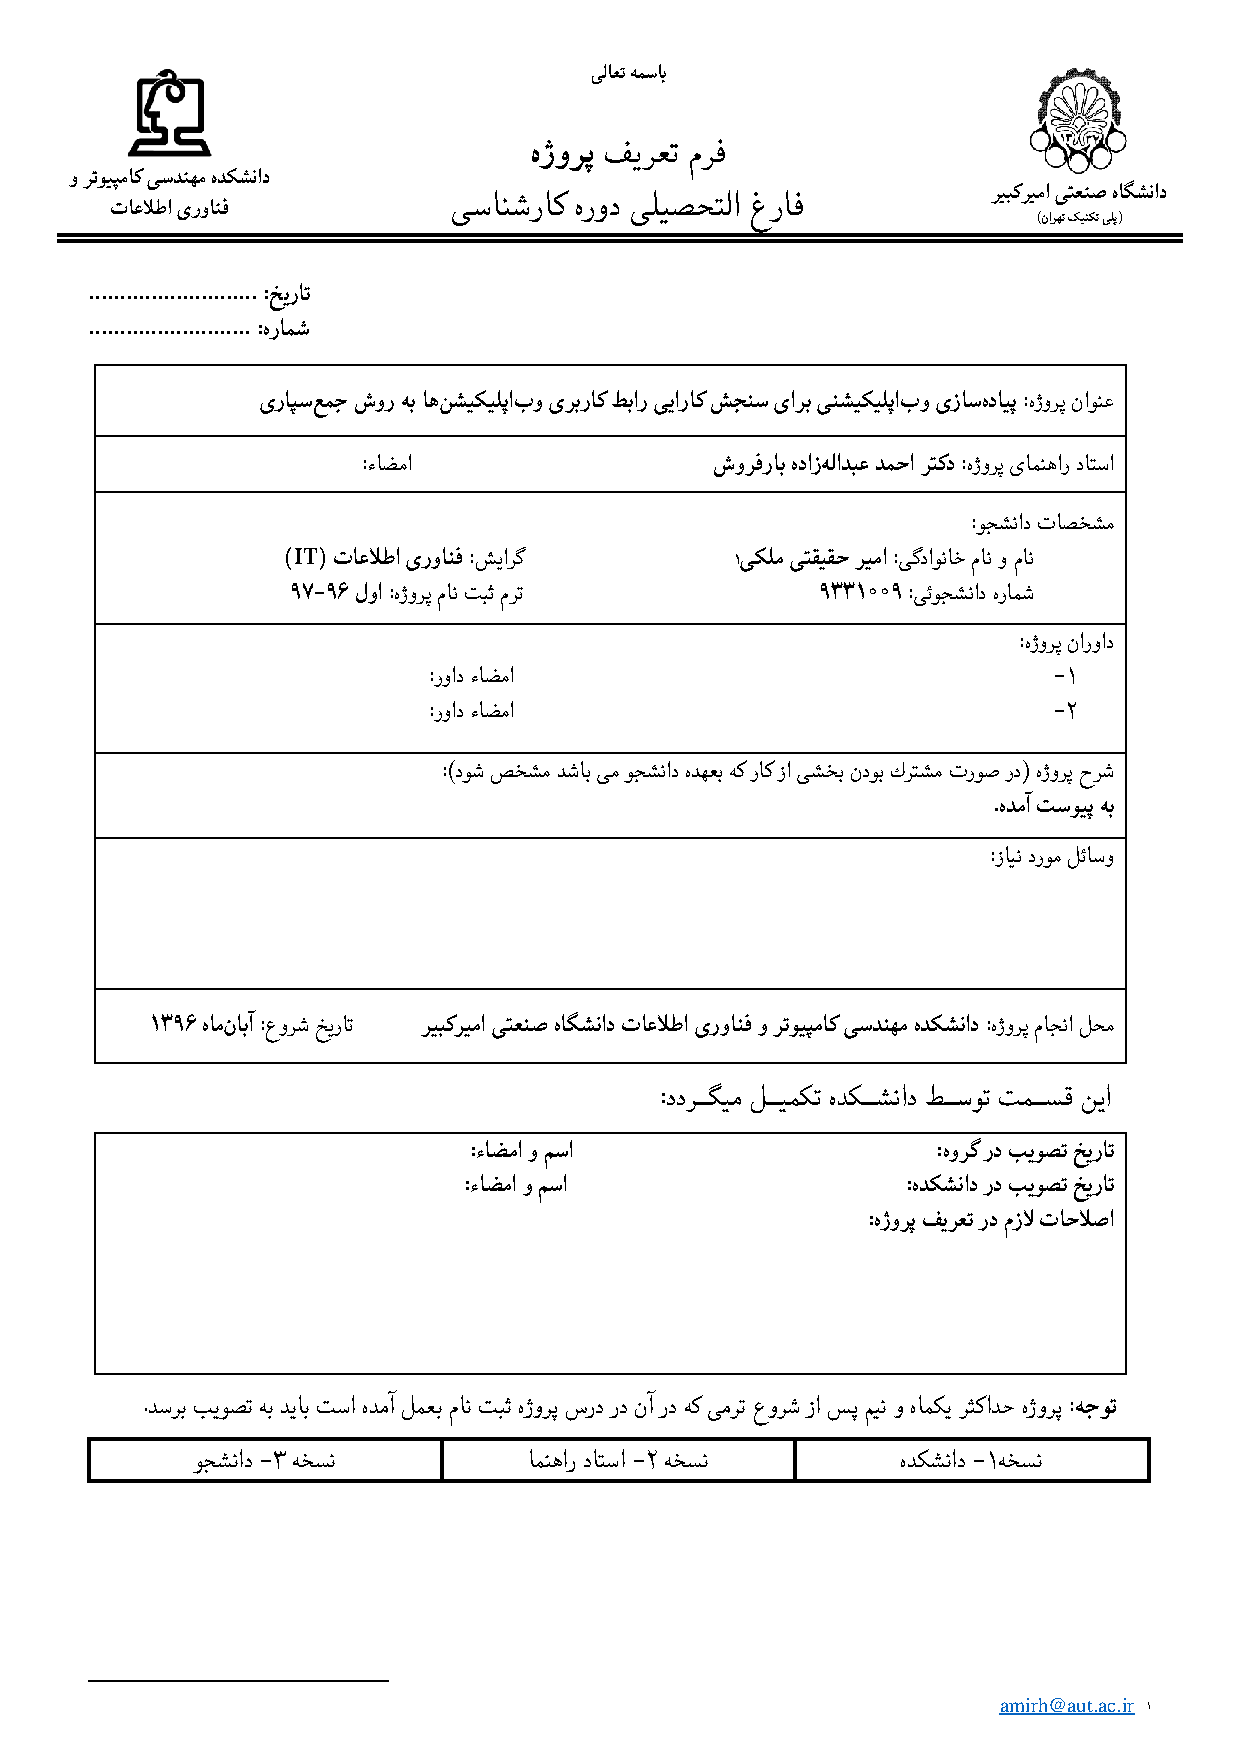
\includepdf[pages=-]{Project_Definition_Page.pdf}
	\end{titlepage}
	\newpage
	\pagenumbering{Alph}
	\begin{abstract}
		\thispagestyle{plain}
	با تقریب خوبی می‌توان گفت تمامی مدل‌های کیفی نرم‌افزار، کارایی را جزو مشخصه‌های اصلی کیفیت یک نرم‌افزار مطرح می‌کنند. وجه مشترک تعاریف متعددی که برای کارایی مطرح می‌شود، در سه بعد کاربر، انجام یک فعالیت مشخص و تعامل با یک واسط برای انجام آن فعالیت، قابل بیان است. به عنوان یک مهندس نرم‌افزار، افزایش کیفیت در محصولات و کاهش هزینه‌های ناشی از خرابی‌ها و یا درخواست‌های تغییر، چالشی تامل برانگیز است. وب‌اپلیکیشن‌ها به عنوان نوعی محصول نرم‌افزاری که در آن‌ها زیبایی، واسط کاربری و نحوه تعامل کاربران مهم است، به دلیل استفاده گسترده‌شان، می‌توانند تاثیر شگرفی در موفقیت یک پروژه صنعتی، کسب‌وکارهای نوپا و یا تسهیل زندگی روزمره با استفاده از نرم‌افزارها داشته باشند. از جمله نقاط ضعف بیشتر وب‌اپلیکیشن‌ها، طراحی نه‌چندان کاربرپسندانه واسط کاربری آن‌هاست که موجب شده تا در بسیاری از موارد، کاربران، علاقه‌مندی استفاده از محصول مبتنی وب یک سازمان را در عین سرمایه‌گذاری‌های زیاد آن سازمان برای جذب کاربر، از دست بدهند و در نتیجه متضرر شوند. گرچه، به صورت ایده‌آل، تمامی تصمیم‌گیری‌های مدیریتی و کلان (از قبیل اتخاذ مدل‌های فرایندی مناسب برای تولید نرم‌افزار با هزینه کم) با نهایت دقت و تجربه انجام می‌شوند، ولی در بسیاری از موارد همچون پروژه تقویم شرکت گوگل، مواردی ملاحظه می‌شود که واسط کاربری ناکارآمد، به ناچار، هزینه‌های گاهاً زیادی به تیم مهندسی نرم‌افزار تحمیل کرده است. با مروری بر منابع مختلف، ارزیابی و تست روی نمونه‌های اولیه رابط کاربری وب‌اپلیکیشن‌ها به منظور رفع نواقص آن‌ها، امری واضح به نظر می‌رسد. اما پاسخ دادن به این سوال که «چه واسط کاربری‌ای خوب است؟» همیشه آسان نبوده و با تغییر فناوری و گذشت زمان شاهد تغییر سریع در نیازمندی‌ها هستیم که شاید چک‌لیست‌ها و توصیه‌ها نیز پاسخگوی دقیقی برای آن‌ها نباشند. بنابراین می‌بایست در طراحی واسط کاربری، به یک روش کمی و قابل استناد، نیازمندی‌ها را با استفاده از نمونه‌های اولیه بسنجیم (که به دلیل هنری انگاشتن اکثر کارها، این امر نادیده گرفته می‌شود). اما سنجش دقیق، نیازمند جمع‌آوری داده از ارزیابی و تست واسط کاربری توسط کاربران نهایی است تا بتوان تحلیل دقیق انجام داد و مشکلات طراحی واسط را به درستی تشخیص داد. یکی از روش‌های جمع‌آوری داده، استفاده از جمع‌سپاری است. باید توجه داشت که استفاده از جمع‌سپاری چالش‌هایی را فرارویمان خواهد گذاشت که از جمله آن‌ها میتوان به عدم وجود صحت در داده‌ها اشاره کرد. در این پروژه وب‌اپلیکیشنی به منظور ارائه داشبورد مدیریتی برای صاحبان طراحی و افراد متمایل به انجام تست‌های مختلف با معیارهای متفاوت و دلخواه، پیاده خواهد شد. همچنین دادگان و پاسخ‌ها و تحلیل‌های تست اپلیکیشن در مواجهه کاربران واقعی با آن‌ها، به اطلاع کاربر خواهد رسید؛ علاوه بر موارد فوق، قسمت اصلی این پروژه در پاسخ به چالش صحت داده در روش جمع‌سپاری، ابتدا رفتار کاربران پاسخ‌دهنده (کارگران) توسط ماتریسی مدل می‌شود که برای مدل‌سازی و به دست آوردن مقادیر مدل‌ها، از روش تزریق سوالات طلایی استفاده خواهد شد. سپس در صورت پایین بودن کیفیت کار کارگران از حد مشخصی که در هنگام مدل‌سازی مشخص می‌شود، نتیجه کار آن‌ها به عنوان داده نامربوط شناخته شده و حذف می‌گردد. امکان تعریف تست‌های دلخواه و محدود نبودن به تست‌های از پیش تعریف شده تفاوت عمده ابزار کارا با سایر ابزارهای مشابه است؛ از جمله ابزارهای مطرح موفق در این حوزه، می‌توان به UsabilityHub، Optimizely و CrazyEgg اشاره کرد که همانطور که ذکر شد، در طی این پروژه، سعی بر برطرف‌سازی برخی از نواقص آن‌هاست.
	\end{abstract}
	\newpage
	\pagenumbering{gobble}
	\tableofcontents
	\newpage
	\pagenumbering{arabic}
	\section{تعریف مسئله}
خریداری یا استفاده از یک محصول با این پیش‌زمینه و تفکر که محصول مورد نظر نیاز خاصی را برطرف خواهد کرد، خود به خود انتظار برطرف کردن نیازمندی‌های مورد نظر را در کاربر می‌انگیزد
\cite{abdollahzade}.
یک محصول نرم‌افزاری موفق نیز به منظور جذب حداکثری کاربران و موفقیت بیش از پیش، می‌بایست از کیفیت بالایی برخوردار باشد. در اپلیکیشن‌های مبتنی بر وب و موبایل که جامعه کاربریشان هر روز بیشتر و بیشتر می‌شود، نیازمندی‌های مختلفی در طول چرخه عمر نرم‌افزار بروز پیدا می‌کنند. به طور کلی در نرم‌افزار،  گسترده‌تر شدن دامنه دسترسی به یک محصول نرم‌افزاری، الزاماتی برای آن فراهم می‌آورد که برای مثال، می‌توان گفت محصول نرم‌افزاری می‌بایست توسط یک فرد عادی از جامعه هدف مشتریان، قابل استفاده باشد. قابل استفاده بودن را نه در دانش فنی کاربران سیستم، بلکه در قابل فهم بودن رابط میان سیستم و کاربران تعریف می‌کنیم
\cite{measuring}.
البته ناگفته نماند دانش فنی بخش غیرقابل اغماضی از توانایی استفاده از یک محصول نرم‌افزاری را ممکن می‌سازد؛ ولی در مورد محصولات نرم‌افزاری تحت وب که به طور معمول با تعداد کاربران زیادی مواجه هستند، قابل استفاده بودن و کارایی 
\footnote{Usability}
آن‌ها در هنگام کار یک کاربر عادی، یکی از معیارهای مهم کیفیت به شمار می‌رود.
	\subsection{کارایی}
به تعبیر نویسندگان مرجع
\cite{measuring}
هر نفر می‌تواند برای خودش تعریفی از کارایی ارائه نماید. در اینجا به ارائه چند نمونه اصلی از تعریف کارایی می‌پردازیم:
\begin{itemize}
	\item
	سازمان بین‌المللی استانداردها (ایزو ۹۲۴۱-۱۱) کارایی را در سه حوزه به این شرح که «میزان سودی که استفاده از یک محصول در رسیدن به اهداف مورد نظر کاربران در رابطه با کاربردی مشخص، که همراه با تاثیرگذاری، بهره‌وری و رضایت باشد، کارایی آن محصول نامیده می‌شود.»
	\item 
	جامعه متخصصین کارایی
	\footnote{\lr{Usability Professionals Association}}
	بیشتر روی فرایند تولید و توسعه محصول تمرکز می‌کنند و با بیان کارایی به عنوان یک روش برای کاستن هزینه‌ها و ابزارهایی که مختص کاربرانشان باشد، از ویژگی مرتبط بودن همواره کارایی با کاربران، استفاده می‌کند.
	\item 
	استیو کورگ در کتاب خود، «کاری نکن که من به فکر کردن بیفتم»
		\cite{don't make me think}،
	تعریف عامیانه‌تری را ارائه می‌دهد. وی معتقد است که کارایی به معنی اطمینان حاصل کردن از کار کردن خوب محصول نهایی است. با این توضیح که یک فرد با دانش، توانمندی و تجربه کم نیز بایستی بتواند از محصول به راحتی استفاده کند و نیازهای خود را برطرف سازد.
\end{itemize}
تمامی تعاریف مطرح برای کارایی، شامل سه زمینه کلیدی و مهم هستند:
\begin{itemize}
	\item کاربری وجود دارد.
	\item این کاربر مشغول انجام کاری است.
	\item این کاربر مشغول انجام کاری با یک سیستم یا محصول نرم‌افزاری است.
\end{itemize}
اینکه کاربر در طول دوره کاری‌اش با سیستم به طور دقیق به چه موارد منفی یا مثبت یا حتی خنثی برخورده، نقش مهمی در تجربه کاربری وی دارد. \\
کارایی به طور کلی به توانایی کاربر در انجام یک کار مشخص با موفقیت دلالت دارد، در حالی که تجربه کاربری به جنبه وسیع‌تری پرداخته و شامل احساسات، عواطف و ادراکات کاربر در حین کار با سیستم می‌شود
\cite{measuring}.
با بررسی مدل‌های کیفی مختلف که به منظور سنجش کمی کیفیت نرم‌افزار ارائه شده‌اند، مشاهده می‌شود که کارایی نرم‌افزار، به عنوان یکی از مشخصه‌های اصلی در اغلب این مدل‌ها به صورت صریح  بیان شده است. مدل‌های مک‌کال، Dromey، ایزو ۹۱۲۶، FURPS و ایزو ۲۵۰۱۰ از مدل‌های اساسی و مدل‌های برتوئا، گکوآمو، آلوارو و راواشد از جمله مدل‌های خاص منظوره‌ای هستند که در آن‌ها کارایی نرم‌افزارها به صورت صریح به عنوان یک فاکتور اصلی بیان شده است 
\cite{pressman}.
همچنین مفهوم کارایی نرم‌افزار به طور ضمنی در بطن اجزای سایر مدل‌های کیفی نهاده شده است. می‌توان گفت کارایی یک نرم‌افزار، از جمله ویژگی‌های مهم کیفی در دستیابی و کنترل کیفیت نرم‌افزار است.
	\subsection{تضمین و کنترل کیفیت}
همانطور که پرسمن در کتابش
\cite{pressman}
مطرح می‌کند، رسیدن به یک محصول با کیفیت در مهندسی نرم‌افزار، به صورت ضمنی و خود به خود ممکن نیست؛ بلکه نتیجه بازنگری در چهار بعد کلی در فرآیند مهندسی نرم‌افزار و اِعمال مجموعه آن‌ها است: روش‌های مهندسی نرم‌افزار، تکنیک‌های مدیریت پروژه، فعالیت‌های کنترل و تضمین کیفیت نرم‌افزار. طبق این اظهار نظر، با فرض اِعمال شدن روش‌های درست و بهره‌ور مهندسی نرم‌افزار و تکنیک‌های موثر در مدیریت پروژه تولید نرم‌افزار - که با تقریب خوبی هر دو را می‌توان جزو روش‌های مدیریتی و در حوزه تصمیم‌گیری‌های کلان سیستم دانست - بدیهی است که همچنان کنترل کیفیت و تضمین آن، دو بعد فنی و جزئی‌تر رسیدن به نرم‌افزار با کیفیت را تشکیل می‌دهند. بنابراین می‌بایست روش‌های موثر به منظور انجام فرایند‌های کنترل کیفیت و تضمین رسیدن به آن، توسط تیم مهندسی نرم‌افزار اتخاذ شود.
اما، مشابه هر فرایند و فعالیت دیگری، رسیدن به کیفیت نیز هزینه‌های خاص خود را دارد. هزینه کیفیت در نرم‌افزار، مطابق اظهارنظر پرسمن، به سه دسته هزینه‌های پیش‌گیری، هزینه‌های ارزیابی و هزینه‌های خرابی تقسیم می‌شود
\cite{pressman}.
هرکدام از این هزینه‌ها، در صورت پیش‌بینی و رفع نواقص محتمل/پیش‌آمده در هر مرحله از طراحی و پیاده‌سازی، بدون اینکه وارد مرحله بعدی شویم، می‌تواند به شدت کاهش یابد 
\cite{pressman}
.
\subsubsection{رابط کاربری، کاهنده یا افزاینده کیفیت؟}
یکی از علل عدم رضایت کاربران و مشتریان از وب‌اپلیکیشن‌ها - که درنتیجه این نارضایتی، آمار کاربران وب‌اپلیکیشن‌های کسب‌وکارها دستخوش تغییرات نامطلوب شده و حتی هزینه‌های گزافی به تیم مهندسی نرم‌افزار به خاطر اعمال تغییر پس از تحویل، وارد می‌شود- طراحی نه‌چندان کاربرپسندانه واسط کاربری و زیبایی آن‌هاست
\cite{assesing}
؛ بدیهی است که استفاده از مدل‌های فرایندی چابک می‌تواند در کاهش هزینه‌های طراحی مجدد پس از تحویل و یا اعمال تغییر در رابط کاربری موجود، موثر باشد 
\cite{pressman}
، اما هنوز یک سوال بدون پاسخ خواهد ماند: چه رابط کاربری‌ای برای کاربران وب‌اپلیکیشن (محصول) من مناسب است و طبق نیازمندی‌های فعلی حداکثر کیفیت را تامین خواهد کرد؟ برای پاسخ به این سوال، چک‌لیست‌ها و توصیه‌های فراوانی
\cite{pressman, sommerville}
ارائه شده است که هرکدام به نحوی در افزایش کیفیت رابط‌های کاربری تاثیرگذار بوده‌اند
\cite{measuring}
، اما برای تست یک رابط کاربری به صورت کمی، تحلیل و یافتن نقاط ضعف، به نظر می‌رسد که بررسی بیشتری مورد نیاز است.
\subsection{کارایی در طراحی رابط کاربری وب اپلیکیشن‌ها}
کارایی در وب‌اپلیکیشن‌ها - که امروزه نقش مهمی در ارائه محتوا و سرویس به کاربران دارند - به عنوان یکی از ابعاد و مشخصه‌های اصلی و مهم در کیفیت مطرح است
\cite{pressman}
. یکی از عوامل بسیار تاثیرگذار در کارایی هر محصولی، رابط کاربری آن است، همچنین کیفیت و چگونگی طراحی رابط کاربری حتی می‌تواند به مرگ و زندگی افراد ختم شود
\cite{measuring}
. پرواضح است که هرچه مشکلات و نواقص رابط‌های کاربری زودتر پیدا شده و مرتفع گردند، با پرداخت هزینه (تلاش و زمان) کمتر به کیفیت بیشتری رسیده‌ایم.
\subsubsection{چرخه طراحی واسط کاربری وب‌اپلیکیشن‌ها}
از جمله مراحل هرم طراحی وب‌اپلیکیشن
\cite{pressman}
، طراحی واسط کاربری است.  همانطور که در شکل
\ref{pyramid}
مشاهده می‌شود، طراحی زیبایی، محتوا، پیمایش، معماری و همچنین مولفه نیز در فرایند طراحی می‌بایست انجام شوند که هرکدام نکات خاص خود را دارند و می‌توانند در کارایی وب‌اپلیکیشن تاثیرگذار باشند.
\begin{figure}[H]
	\centering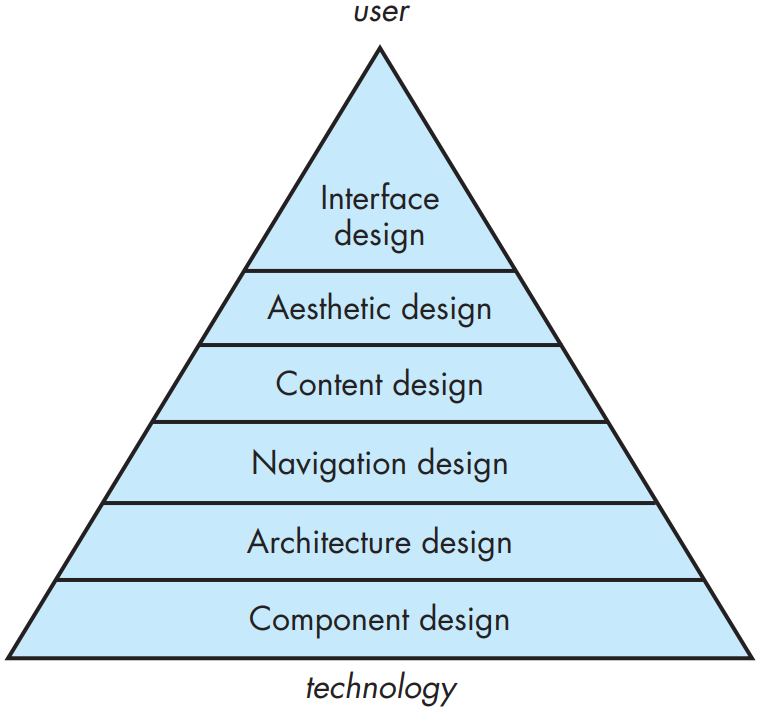
\includegraphics[width=8cm]{Resources/pyramid.PNG}
	\caption{هرم طراحی وب‌اپلیکیشن‌ها
	\cite{pressman}
	}
	\label{pyramid}
\end{figure}
قبل از تولید کد وب‌اپلیکیشن، واسط کاربری، به صورت یک نمونه اولیه و در قالب طرح‌های ابتدایی، ماکت‌های مفهومی و یا چارچوب‌های کلی توصیف و طراحی می‌شوند. پس از رسیدن به توافق با مشتری (در صورت نیاز) و یا اعمال تغییرات متعدد تا رسیدن به توافق، این طراحی به کد قابل اجرا و پیاده‌سازی روی وب‌اپلیکیشن تبدیل می‌شود و نهایتا به تولید واسط کاربری آن می‌انجامد
\cite{sommerville}.

...شکل مورد نیاز است…
مطابق آنچه در قسمت تضمین و کنترل کیفیت گفته شد، در صورت ارزیابی، تحلیل و رفع ایرادات مربوط به کارایی رابط کاربری، در همان مراحل ابتدایی و پس از تولید نمونه‌اولیه، می‌توان هزینه‌های بعدی را به طور قابل ملاحظه‌ای کمتر کرد.
مانند هر روش کیفی دیگری در تضمین کیفیت نرم‌افزار، به منظور دستیابی به کارایی قابل قبول (مطابق نیازهای مشتری) در واسط کاربری وب‌اپلیکیشن‌ها (همچون هر مشخصه اصلی دیگری) می‌بایست فاکتورها، معیارها و مولفه‌های مختلفی به منظور خرد و قابل اندازه‌گیری کردن این مفهوم کلان مطرح شود به طوری که بتوان در قالب مقادیر کمی، نیازمندی‌ها را با داده‌های به دست آمده از ارزیابی رابط کاربری وب‌اپلیکیشن مقایسه و تحلیل کرد. اما در بسیاری از موارد، همانطور که
\cite{assesing, main2}
ذکر می‌کنند، حقیقت محض و یا هیوریستیک تضمین‌کننده‌ای برای رسیدن به یک رابط کاربری «خوب» وجود ندارد و طراحی‌های کارا و موثر موفقیت خود را اغلب یا به روش‌های تجربی، که الزاماً با روش‌های علمی به اثبات نرسیده‌اند، و یا به ذوق هنری طراح مدیون‌اند
\cite{measuring}.
\subsection{جمع‌سپاری}
در سال ۲۰۱۲، با بررسی‌های مرجع 
\cite{estelle}
، حدود ۴۰ تعریف مختلف در مقالات و پژوهش‌های علمی، حتی گاهی تعاریف متناقض با هم، برای جمع‌سپاری ارائه شده است. نویسندگان آن اثر، با درنظر گرفتن ابعاد مطرح در تعاریف مختلف، در نهایت تعریف نسبتا مفصلی از این مفهوم ارائه می‌دهند که ترجمه آزاد آن در ادامه ذکر شده است: \\
\paragraph{جمع‌سپاری}
جمع‌سپاری\footnote{Crowdsourcing}
نوعی فعالیت برخط مشارکتی است که طی آن یک فرد، یا یک سازمان با ابزارهای کافی به گروهی از افراد با سطح دانش متغیر و گونه‌های متفاوت و با تعداد نامعلومی به انجام فعالیت‌هایی می‌پردازند. در این کار دو سر برد، کاربران انجام دهنده کار (کارگارن)  به دلیل داوطلبانه بودن مشارکتشان، از انجام کار خود احساس رضایت می‌کنند؛ چه به خاطر پولی که در ازای انجام کار دریافت می‌کنند و چه به خاطر توسعه مهارت‌های شخصی و یا غیره؛ افراد جمع‌سپارنده هم از مشارکت افراد در حل مسائل پیچیده کمک جسته و سودآوری خود را خواهند داشت. \\
یکی از انگیزه‌های استفاده از جمع‌سپاری، برای جمع‌آوری داده\footnote{Data Collection} است. در این استفاده، از کارگران جمع‌سپاری شده بهره گرفته می‌شود تا بتوان به مجموعه عظیمی از دیتاست‌ها و یا داده‌های جدید دست پیدا کرد.
\subsubsection{جمع‌سپاری برای جمع‌آوری داده}
انگیزه اصلی استفاده از جمع‌سپاری در این پروژه، جمع‌آوری داده است. ابزار هدف، قادر خواهد بود تا با استفاده از جمع‌سپاری، بتواند نتایج تست‌های تعریف‌شده توسط مشتریان را از کارگران جمع‌آوری کرده و روی آن‌ها تحلیل و پردازش انجام دهد. عدم وجود یک حقیقت محض قابل اتکا\footnote{Ground Truth} در رابطه با خوب بودن و یا بد بودن یک طراحی رابط کاربری و سلیقه‌ای بودن آن، مهم‌ترین انگیزه استفاده از جمع‌سپاری است که مبتنی بودن تصمیمات و داده‌ها بر اساس داده‌های کاربران مخاطب، می‌تواند منجر به موفقیت حداکثری یک محصول در سازمان شود.
\section{جزییات فنی سیستم هدف و روش مورد استفاده}
\subsection{نمودار \lr{Use Case}}
ساختار سیستم هدف و اجزای آن که در شکل 
\ref{usecase}
مشاهده می‌شود.
سیستم کارا در نهایت، مشتریان را قادر به آپلود طرح‌های مفهومی، اسکچ‌ها، ماک‌آپ‌ها و طراحی‌های خود خواهد کرد تا با استفاده از آن‌ها، برخی از سناریوهای از پیش تایین شده و یا یک سناریوی دلخواه را برای تست واسط کاربری مورد نظر خود استفاده کنند و با استفاده از جمع‌سپاری، داده‌های نتیجه را جمع‌آوری و تحلیل کرده و درنهایت گزارش‌گیری نمایند.
\begin{figure}[H]
	\centering 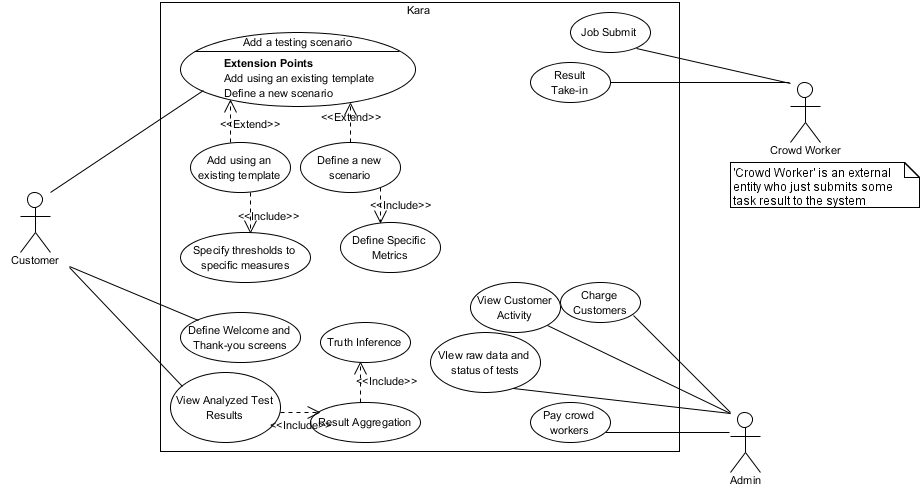
\includegraphics[width=\linewidth]{Resources/UseCase.png}
	\caption{نمودار \lr{Use Case} سیستم هدف}
	\label{usecase}
\end{figure}



\begin{thebibliography}{20}
	\begin{latin}
		\bibitem{pressman}
			R. Pressman and B. Maxim, SOFTWARE ENGINEERING: A PRACTITIONER’S APPROACH, 8th ed. New York: McGraw-Hill Education, 2015.
		\bibitem{main2}
			J. P. Miguel, D. Mauricio and G. Rodríguez, "A Review of Software Quality Models for the Evaluation of Software Products", International Journal of Software Engineering \& Applications, vol. 5, no. 6, pp. 31-53, 2014.
		\bibitem{assesing}
			R. Agarwal and V. Venkatesh, "Assessing a Firm's Web Presence: A Heuristic Evaluation Procedure for the Measurement of Usability", Information Systems Research, vol. 13, no. 2, pp. 168-186, 2002.
		\bibitem{measuring}
			T. Tullis and W. Albert, Measuring the user experience, 3rd ed. Amsterdam: Elsevier, 2013.
		\bibitem{estelle}
			E. Estellés-Arolas and F. González-Ladrón-de-Guevara, "Towards an integrated crowdsourcing definition", Journal of Information Science, vol. 38, no. 2, pp. 189-200, 2012.
		\bibitem{don't make me think}
		S. Krug, Don’t make me think!: a common sense approach to Web usability, 1st ed. Pearson Education India, 2000.
		\bibitem{sommerville}
		I. Sommerville, Software engineering, Tenth edition, Global edition. Boston, Mass. Amsterdam Cape Town: Pearson Education Limited, 2016.
		\bibitem{survey}
		G. Li, J. Wang, Y. Zheng and M. J. Franklin, "Crowdsourced Data Management: A Survey," in IEEE Transactions on Knowledge and Data Engineering, vol. 28, no. 9, pp. 2296-2319, Sept. 1 2016.
		doi: 10.1109/TKDE.2016.2535242
	\end{latin}
	\bibitem{abdollahzade}
	عبداله‌زاده بارفروش، احمد. (۱۳۸۹). کلیات متدولوژی تامین کیفیت. تهران: انتشارات آدینه.
\end{thebibliography}

	
\end{document}